\chapter{Introduction}
\label{chapter:intro}


This thesis introduces a social robot as a teacher of assistive sign language to children with autism. The robot InMoov, which is modified specifically for this use, is used as a platform for research. The thesis answers the question: How should the InMoov be designed to be a tutor of assistive sign language for children with autism? First, design choices that could affect the usefulness of the InMoov as a sign language tutor are examined. An initial, theoretical design is defined according to existing research. In order to achieve this design, a design framework for the design of social robots is introduced. The InMoov is then modified accordingly, and the resulting implementation is examined in experiments with children with autism. The results are examined, based on which recommendations for future implementations of the InMoov in this use are made. Recommendations for robots to be used with autistic children in general are also made.

This introduction details the background and motivation for the research, defines the research problem and three different research questions, discusses the goal and scope of the study, and introduces the structure of the study.

%%%%%%%%%%
%%%%%%%%%%


\section{Background and motivation}


Social robotics is a rapidly growing application area in the field of robotics. Social robots are robots that aim to interact with people in a manner that feels natural and interpersonal, usually to achieve social-emotional goals in diverse fields of application such as communication, collaboration, quality of life, health and education \cite{Breazeal2008}. This study focuses on the domains of rehabilitation and healthcare, as well as education. Application branches of robotics are visible in figure \ref{fig:fieldRobotics}.

\begin{figure}
\centering
  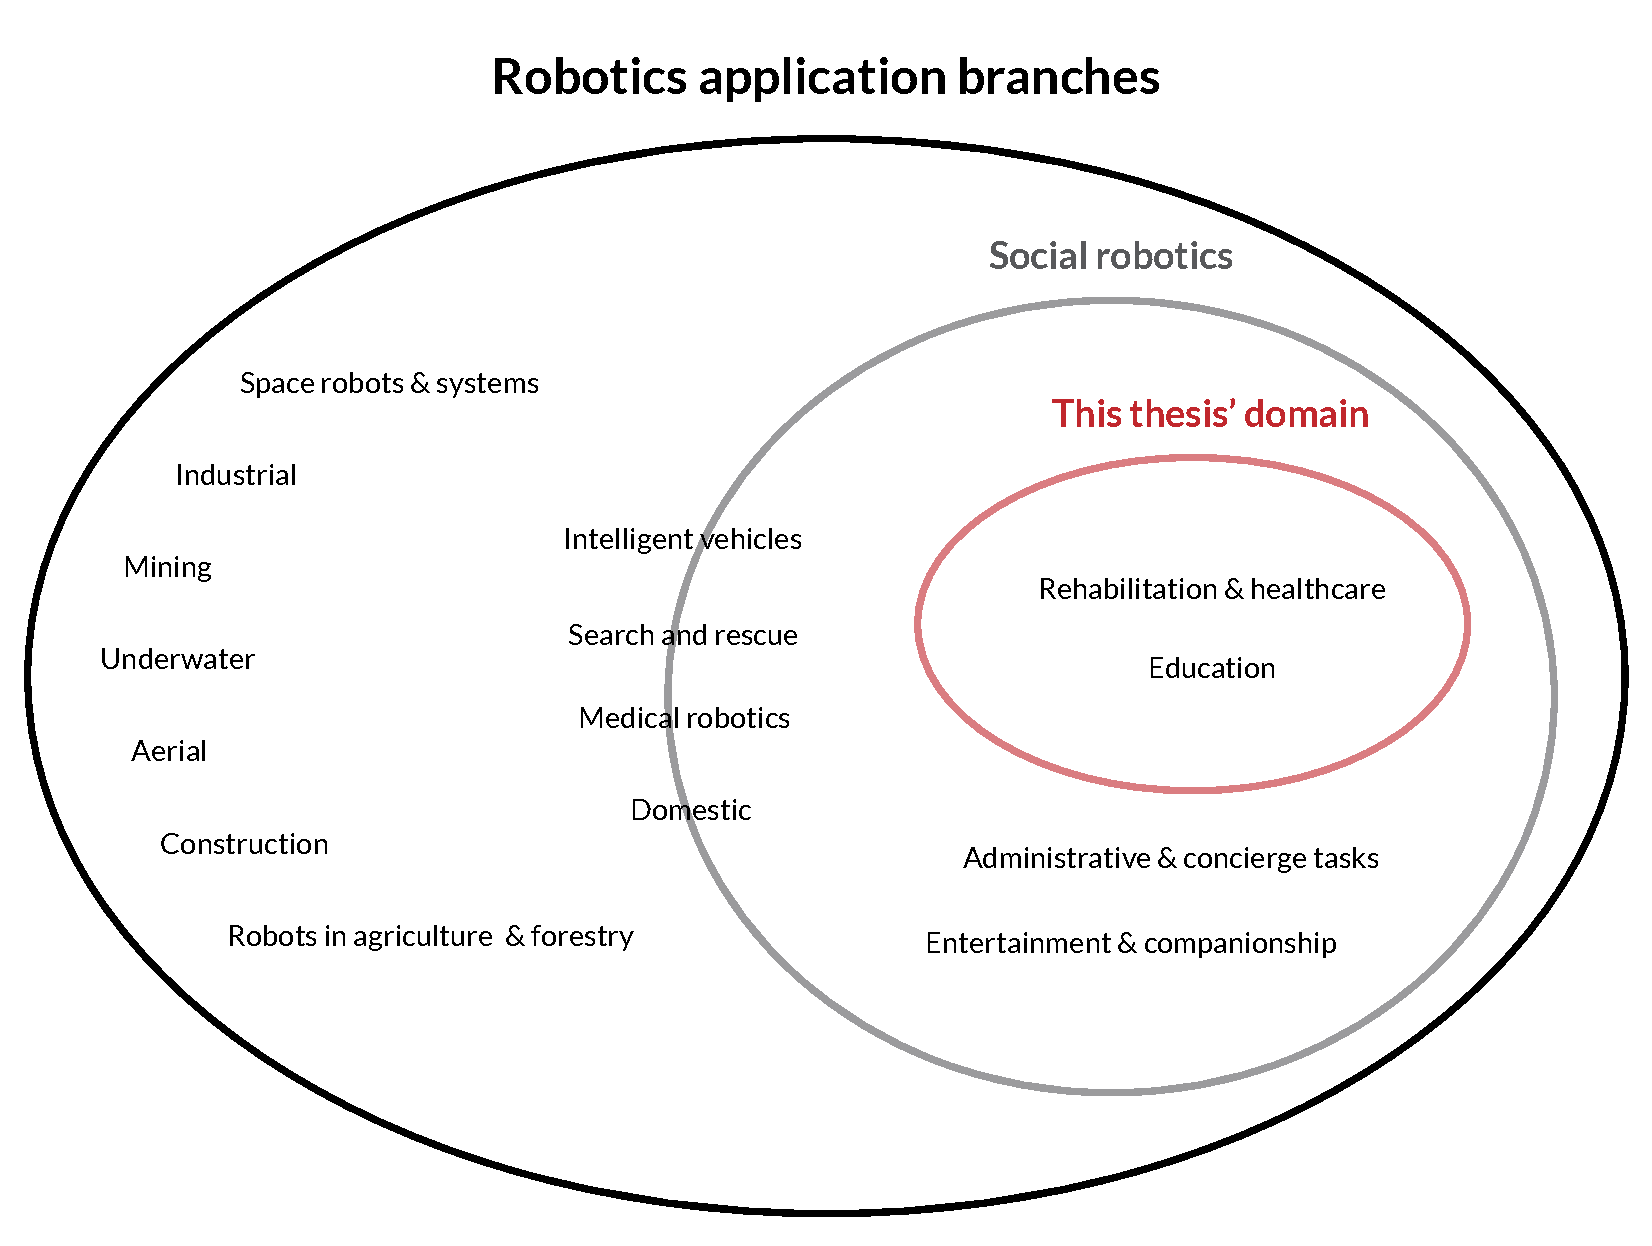
\includegraphics[scale=0.45]{images/robotics_application_branches.pdf}
  \caption{The field of robotics, adapted from \cite{Breazeal2008}. This project focuses on the rehabilitation, healthcare and education domains of robotics. Intelligent vehicles, search and rescue robotics, medical robotics and domestic robotics can be considered to be on the border of being social, which is why they are depicted partially inside the sphere of social robotics.}
  \label{fig:fieldRobotics}
\end{figure}

Autism spectrum disorder (ASD) is a disorder characterized by impaired language and communication, impaired social behavior, and narrow flexibility in daily activities \cite{frith2003autism, tetzchner, WHOautism}. Assistive sign language is a form of communication used by people with autism with limited verbal abilities \cite{puheSuomi}. Autists usually learn assistive signs early on, which is why this research examines autistic children specifically. 

Robots have been previously explored in communication therapy use with children with autism. The rationale behind using a robot for this type of therapy is that the robot's social behavior can be consistently controlled, which may make it less overwhelming for autistic people \cite{kozima2009keepon}. Additionally, children with ASDs have been observed to show more attention toward objects than to humans \cite{autismi}, and to be more interested in treatment when it involves robotic components \cite{robins2006appearance}. Research has been conducted to explore robots as tools in communication therapy for autistic children \cite{ARIA, charlie2011, boccanfuso2017low, duquette2008exploring, giullian2010detailed, goodrich2012incorporating, kim2013social, kim2015potential, kozima2009keepon,pop2013social, robins2004effects, robins2006appearance, wainer2014pilot}, and separately to teach sign language to neurotypical children \cite{taleofarobot, uluer2015new}. Combining these two elements served as the motivation to conduct this research. 

In order to examine whether a robot teaching assistive sign language to children with autism is feasible, experiments are performed with autistic children. The robot used as a platform for this solution is the open source robot InMoov, which is modified to be appropriate for this use. The InMoov is a human-sized humanoid robot torso, constructed out of 3D printed body components and gears. Its entire schematic is available under the Creative Commons license (CC-BY-NC). The original InMoov schematic was designed by Gael Langevin, and further contributions to its schematics and attached software are made by the open source community of InMoov enthusiasts \cite{inmoov}. The InMoov was selected due to availability, and to my knowledge has not been used in other academic studies.

The experiments are done in collaboration with the Satakunta hospital district in Finland. Two professionals working at the Satakunta hospital district acted as advisors for the design process presented in this thesis. These experts consulted are a speech therapist, Akuliina Lehtonen, and a neuropsychologist, Terhi Nyman. 

%%%%%%%%%%
%%%%%%%%%%


\section{Research problem}

This thesis aims to design and implement the first instance of a robot teaching assistive sign language to children with autism. This thesis explores the research problem:

\vspace{3mm}
\noindent\textbf{How should the InMoov be designed to be a tutor of assistive sign language for children with autism?}
\vspace{3mm}

This is done by first developing an understanding of autism, assistive signing, and robots in use by children with autism. With the developed knowledge, a design is constructed and tested with autistic children. This design is then evaluated. Thus, the research problem is divided into three research questions:


\vspace{3mm}

\noindent\textbf{RQ1: What are the design choices that may impact the InMoov's usefulness as a sign language tutor?}
\vspace{3mm}

\noindent\textbf{RQ2: Is the designed robot successful as an assistive sign tutor?}
\vspace{3mm}

\noindent\textbf{RQ3: How should the initial design or consequent designs be modified?}
\vspace{3mm}


The knowledge necessary to answer RQ1 is gathered in chapter \ref{chapter:background}, after which a design is constructed in chapter \ref{chapter:design}. The methods to answer RQ2 are detailed in chapter \ref{chapter:methods}, and results are examined in chapter \ref{chapter:results}. RQ3 is discussed in chapter \ref{chapter:discussion}.


%%%%%%%%%%
%%%%%%%%%%

\section{Objectives and scope of the thesis}

The objective of this thesis is to provide knowledge on the design of social robots, specifically for use in teaching assistive sign language to children with autism. 

On an empirical level, this objective is fulfilled by detailing the first pilot study of a robot teaching assistive signs to children with autism. The study examines whether the robot is successful as a tutor. Specifically, three different design conditions are compared, in order to provide knowledge on which of these three design decisions are beneficial. Additionally, future recommendations for the robot presented in this thesis, and other similar robots that could be implemented in the future, are presented based on the results from the experiments. These recommendations can help people designing robots make decisions in the future.

On a theoretical level, the objective is fulfilled by proposing a design framework for the design of social robots. Existing social robots have not been systematically and consistently designed from end-to-end, which motivated the creation of the framework. The framework is utilized as a tool during the design process presented in this thesis, and it can be utilized in the design of any social robot in the future. To my knowledge, this is the only design framework that details the entire design process of a social robot. In this thesis, the framework is used specifically to modify the design of the robot InMoov to be suitable for teaching assistive signs to children with autism. The description of this process serves as an example of how the framework can be utilized.

Due to the large base of theoretical knowledge that is presented in this thesis, the experiments themselves are kept small in size. Additionally, organizing experiments with autistic children is challenging, which is why only 10 participants' data are analyzed. To provide definitive results on the usefulness of a robot in this type of use, clinical level studies would need to be conducted. However, due to the pilot nature of the study, a small number of participants is deemed as useful to provide the first steps into a previously unknown niche branch of robotics.

Due to the narrow scope of the experiment itself, the design framework is considered as the most important contribution of this thesis.


%%%%%%%%%%
%%%%%%%%%%

\section{Structure of the thesis}

The second chapter is a literature review presenting academic literature on autism and the communication impairment associated with it, social robots previously in used in communication therapy, and social robots previously used as teachers of sign language. The chapter ends with the theoretical knowledge being synthesized into design guidelines for the robot.

Following the discussion of the background, the design for the robot is presented. A design framework is introduced as a tool to make design decisions about different dimensions of a social robot. In this thesis, the robot InMoov is situated into the design framework, and modifications are made to it according to the design guidelines established in chapter \ref{chapter:background}.

Chapter \ref{chapter:methods} presents the methods to be used to study the modified InMoov teaching assistive signs to children with autism. The research setting, process and methodology are presented.

Results of the experiments are presented in chapter \ref{chapter:results}. Both quantitative and qualitative results are analyzed.

Following the results of the study, the chapter \ref{chapter:discussion} discusses the answers to the research questions. Limitations of the study are detailed thoroughly. Practical and theoretical implications, as well as suggestions for future research are discussed. Finally, a conclusion is provided.
